\subsection{Peak performance}
\label{subsec:peak_fp}
Rosa's nodes are equipped with dual-socket Intel Xeon E5-2650 v3 processors, 10 cores and AVX2 units that operates with 256-bit vectors\cite{intel-e5-2650v3,usi-rosa-hardware}. Haswell micro-architecture have two 256-bit FMA instructions per cycle meaning that each core performs four double-precision at 2.30~GHz \cite{intel-optimization-manual}.

The Rosa documentation (and also the output from command \texttt{sinfo} \ref{lst:sinfo}) shows 42 compute nodes (icsnode01--icsnode42).\cite{usi-rosa-hardware} \\ 
The calculations for the aggregate peak throughput for the partition is written in the provided file \href{run:../src/2-Performance-characteristics/01/INTEL_XEON_E5-2650.txt}{[INTEL\_XEON\_E5-2650.txt]} in the \href{run:../src/2-Performance-characteristics/02/}{02} folder and reported here below:

\lstinputlisting[
    caption={Peak throughput breakdown for Intel Xeon E5-2650 v3},
    captionpos=b,
    label={lst:e5-2650-peak},
]{../src/2-Performance-characteristics/01/INTEL_XEON_E5-2650.txt}


\subsection{Memory Hierarchies}
\label{subsec:memory_hierarchy}

In order to study the memory hierarchy of Rosa compute nodes, I used the commands: \texttt{lscpu}, \texttt{cat /proc/meminfo}, and \texttt{hwloc-ls}. The complete output files are available in the submission in the folder \href{run:../src/2-Performance-characteristics/02/}{02}.

The results are summarized in Table~\ref{tab:memory_hierarchy}.

\begin{table}[h]
    \centering
    \begin{tabular}{|l|r|}
    \hline
    \textbf{Component} & \textbf{Size} \\
    \hline
    Main memory (total) & 62 GB \\
    Main memory (per NUMA node) & 31 GB \\
    L3 cache (shared per socket) & 25 MB \\
    L2 cache (per core) & 256 KB \\
    L1d cache (per core) & 32 KB \\
    L1i cache (per core) & 32 KB \\
    \hline
    \end{tabular}
    \caption{Memory hierarchy of Rosa compute node}
    \label{tab:memory_hierarchy}
\end{table}

The graphical representation of the memory hierarchy is shown in Figure~\ref{fig:memory_topology}.

\begin{figure}[h]
\centering
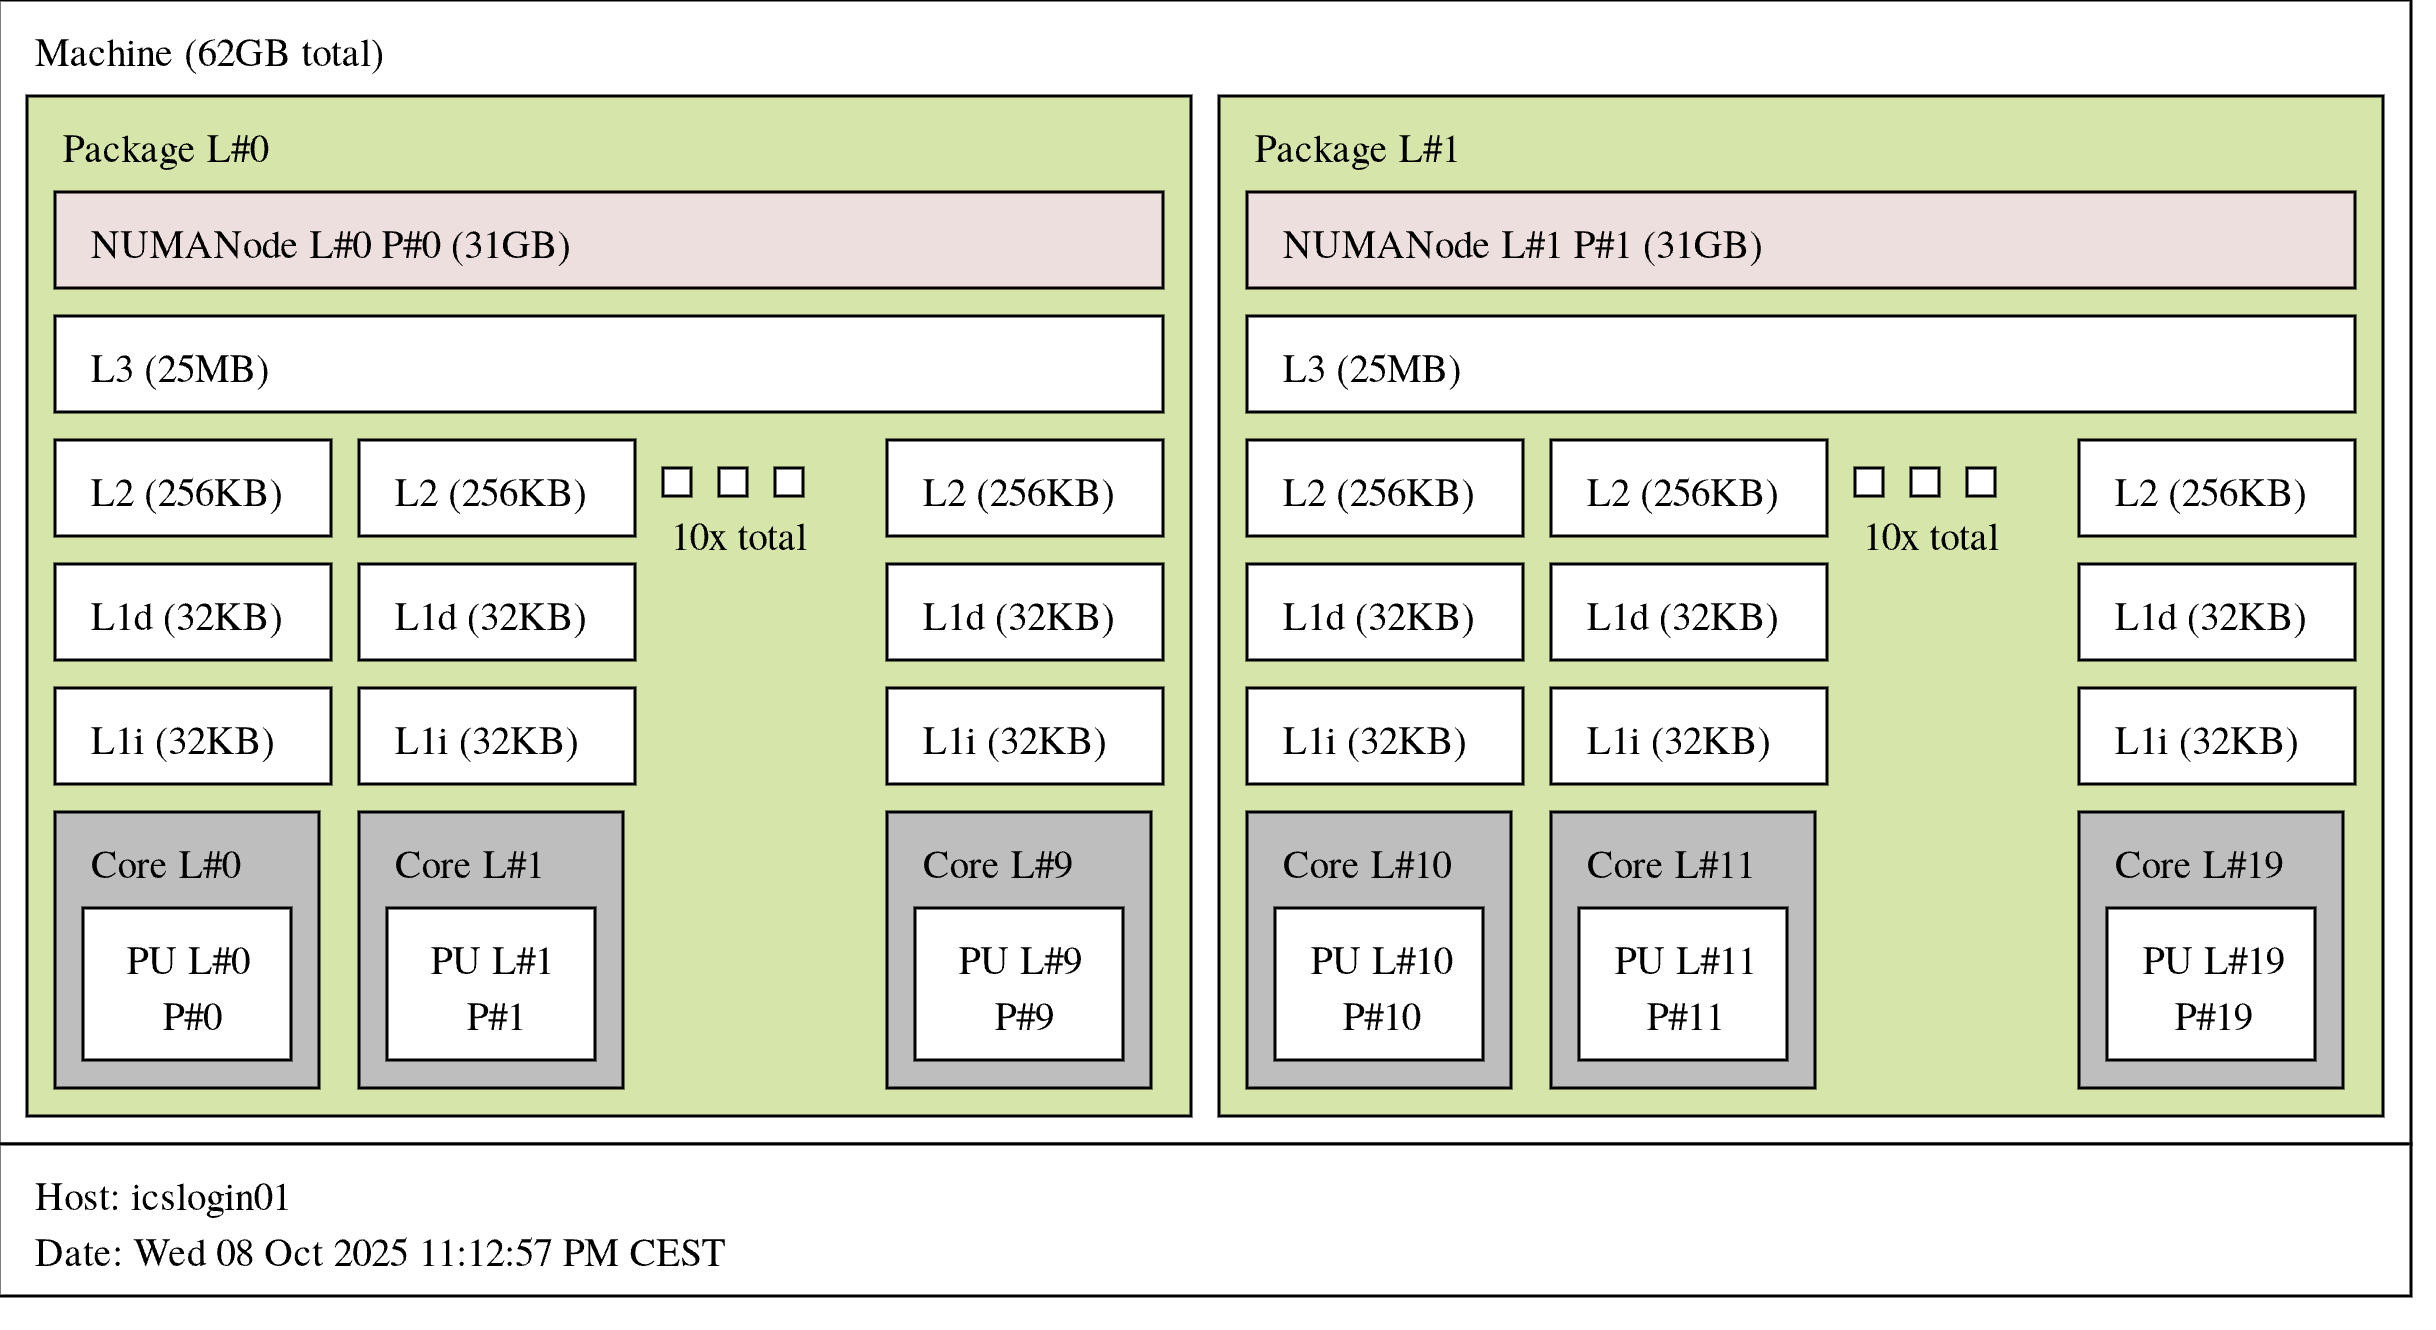
\includegraphics[width=0.9\textwidth]{../src/2-Performance-characteristics/02/XEON_E5-2650.png}
\caption{Graphical representation of Rosa node topology generated by command \texttt{hwloc-ls}.}
\label{fig:memory_topology}
\end{figure}

\subsection{Bandwidth: STREAM benchmark}


\subsection{Performance model: A simple roofline model}